\documentclass{article}
\usepackage[12pt]{extsizes}
\usepackage[utf8x]{inputenc}
\usepackage[russianb]{babel}
\usepackage{vmargin}
\usepackage{blindtext}
\setpapersize{A4}
\usepackage{relsize}
\setmarginsrb{2cm}{1.5cm}{1cm}{1.5cm}{0pt}{0mm}{0pt}{13mm}
\usepackage{indentfirst}
\usepackage{graphicx}
\usepackage{amsmath}
\usepackage{amssymb}
\usepackage{amsthm}
\usepackage{algorithm}
\usepackage{algpseudocode}
\usepackage{ mathrsfs }
\usepackage{amsmath}
\bibliographystyle{unsrt} 
%\usepackage{biblatex}
\renewcommand{\baselinestretch}{1.3}


\makeatletter
\newcommand{\doublewidetilde}[1]{{%
  \mathpalette\double@widetilde{#1}%
}}
\newcommand{\double@widetilde}[2]{%
  \sbox\z@{$\m@th#1\widetilde{#2}$}%
  \ht\z@=.9\ht\z@
  \widetilde{\box\z@}%
}
\makeatother




\newtheorem{thm}{Теорема}[section]
\newtheorem{lm}{Лемма}[section]
\newtheorem{df}{Определение}[section]
\newtheorem{cor}{Следствие}[section]
\newtheorem{mrk}{Замечание}[section]


\begin{document}

\titlepage 


	\thispagestyle{empty}
	
	\begin{center}
		\ \vspace{-1cm}
		
		
\includegraphics[width=0.4\textwidth]{msu_logo_small.png}\\
		\textsc { Московский государственный университет имени М.~В.~Ломоносова\\
		Факультет вычислительной математики и кибернетики\\
		Кафедра математической физики}
		
		\vfill
		
		\Large{ Турганбаев Сатбек Амангельдыулы}
		
		\vspace{1cm}
		
	       \LARGE \textbf {Исследование метода восстановления \\волнового фронта по его наклонам на основе вейвлетов Хаара }


		\vspace{1cm}

		\large  {ВЫПУСКНАЯ КВАЛИФИКАЦИОННАЯ РАБОТА }
	\end{center}
	
	\vspace{1cm}
	
	\begin{flushright}
		\large{
		\textbf{Научный руководитель:}\\
		д.ф.-м.н.\\
                Разгулин Александр Витальевич
               }
	\end{flushright}
	
	\vfill
	
	\begin{center}
		\large{Москва, 2018}
	\end{center}


\pagenumbering{gobble}



\newpage

\pagenumbering{arabic}
\tableofcontents



\addtocontents{toc}{\protect\setcounter{tocdepth}{2}}

\newpage


\newpage
\section*{Введение}
\addcontentsline{toc}{section}{Введение}
Методы адаптивной оптики активно используются в настоящее время и получили широкое распространение в различных областях науки и техники. Например системы адаптивной оптики, используемые в современных телескопах обеспечивают работу гибких зеркал для исправления аберраций света звезд, вызванных турбулентностью атмосферы Земли \cite{Tyson}. Также они используются при конструировании сверхмощных лазеров и диагностических медицинских систем. Одной из задач систем адаптивной оптики является измерение волнового фронта. Для решения данной задачи существуют соответствующие устройства, в частности датчик Шака-Гартмана. Датчик Шака-Гартмана измеряет локальные наклоны на дискретном множестве точек. После измерения локальных формируются двумерные матрицы локальных наклонов $g_1$, $g_2$. Возникает задача восстановления волнового фронта по этим матрицам.
Существует несколько подходов для решения поставленной задачи:
\begin{itemize}
\item вычисление псевдообратной матрицы \cite{pseudo_inv1}
\item интегрирование градиентов в частотной области и нахождение обратного преобразования Фурье \cite{fourier_1}
\end{itemize}
В данной работе будут исследованы вейвлет и вариационный методы восстановления волнового фронта. Вейвлет метод был предложен в \cite{new_method1},\cite{new_method2}, вариационный в \cite{vatiational_base}.

Вейвлет метод заключается в использовании преобразования Хаара. Удается получить двумерное разложение по вейвлет разложение исходного волнового фронта, путем фильтрации $g_1$, $g_2$. Когда $g_1,\,g_2$ являются производными вперед по $x,\,y$ в декартовой системе координат, удается получить дискретное вейвлет преобразование исходного волнового фронта, а затем и сам волновой фронт с помощью обратного преобразования. Метод позволяет работать с матрицами произвольных размеров. Это важное свойство ввиду того, что современные датчики Шака-Гартмана состоят из больношо числа микролинз, их количество может превышать 10000. 
В работе будет рассмотрена работа метода на поверхностях, представленных полиномами Цернике, при различных представлениях $g_1,\,g_2$.

В вариационном методе задача восстановление формулируется в виде задачи минимизации целевого функционала невязки между производными искомой функции по $x,\,y$ и соответствующими наклонами волнового фронта $g_1,\, g_2$. Метод заключается в построении проекционно-разностной схемы и решении её методом Фурье. Будет рассмотрена работа метода на полиномах Цернике, при различных представлениях $g_1,\,g_2$. В отличие от \cite{vatiational_base}, будут рассмотрены $g_1,\,g_2$ в виде средних локальных апертур значений наклонов,а также получена соответствующая частотная характеристика.
\newpage

\section{Постановка задачи}
Рассмотрим производную от двух переменных $u(x,y)$ , ее производные имеют вид  $u_x(x,y)$, $u_y(x,y)$.
Введем сетку: 
\begin{equation}
\omega_h = \{(x_i, y_j) \,:\, x_i = ih_1,\,y_j = jh_2,\, i = 0..N_1,\, j = 0..N_2;\; h_{1,2}N_{1,2} = 2\pi\}
\end{equation}
Матрицы $U,\, g_1,\, g_2$ являются дискретными представлениями функций $u(x,y) ,\, u_x(x,y) ,\, u_y(x,y)$ на сетке $\omega_h$. Задача восстановления волнового фронта состоит в приближенном восстановлении  матрицы матрицы $U$, по известным наклонам $g_1,\, g_2$.

Представление $g_1 ,\, g_2$ может быть разным и существенно влияет на работу рассматриваемых методов. Далее будут рассмотрены следующие случаи: разностные производные, точные значения наклонов в узлах, средние значения наклонов по локальным апертурам. Заметим, что последний способ представления наклонов волнового фронта наиболее адекватно моделирует данные, снимаемые с датчиков Шака-Гартмана.

В вейвлет методе обычно предполагается, что $g_1, g_2$ являются разностными производными вперед по $x,\,y$ в точках сетки. Проекционный может быть модифицирован для различных $g_1, \, g_2$.
\section{Вейвлет метод восстановления волнового фронта}
\subsection{Преобразование Хаара} 
Преобразование Хаара используется для сжатия входных сигналов, компрессии изображений, в основном цветных и черно-белых с плавными переходами. Идеален для изображений типа рентгеновских снимков. Данный вид архивации известен довольно давно и напрямую исходит из идеи использования когерентности областей.
\subsubsection{Формулировки и определения}
\textbf{Z-преобразованием} дискретного сигнала $\{s_j\}_{ j \in Z}$ называется полином Лорана 
$P_{s}(z) = \sum  \limits_{j \in Z} s_{j}z^{-j}$.
$h = (\frac{1}{\sqrt{2}}, \frac{1}{\sqrt{2}}),~g = (\frac{1}{\sqrt{2}}, -\frac{1}{\sqrt{2}})$ - низкочастотный и высокочастотный фильтры преобразования Хаара.
$$ H_{L}(z) = \frac{1 + z^{-1}}{\sqrt{2}} \;\; H_{H}(z) = \frac{1 - z^{-1}}{\sqrt{2}} $$
$H_{L}(z)$,~$H_{H}(z)$ - z - преобразования фильтров $h$ и $g$ соответственно.

\textbf{Линейной сверткой} двух дискретных сигналов $a(n),~ n=0 \ldots N-1$ и $b(n),~ n=0 \ldots M-1$ называется выражение:
$$ h = a \otimes b; \;\; h(n) =  \sum_{m=0}^{n} a(m)b(n-m) $$
В ввиду того, что сигналы конечномерные на границах возникает неопределенность из-за отсутствия соответствующих элементов. Проблема решается различными способами: дополнение одного из обоих сигналов $0$-ми, константами, симметричное отражение и т.д.

Также одним из свойств $z$-преобразования является то, что $z$-преобразование свертки двух сигналов равно произведению $z$-преобразований этих сигналов. 

\textbf{$\uparrow s$} - операция, добавляющая $0$ после каждого элемента сигнала $s$.

\textbf{$\downarrow_k s$} - операция, удаляющая каждый $k$-ый элемент сигнала $s$.

Если $s = (1,2,3,4)$, то $\uparrow_2 s = (1,0,2,0,3,0,4,0)$, а $\downarrow_{2} s = (1,3)$.

Также стоит отметить, что:
$$\downarrow_2 H_L(z^{2^k}) = H_L(z^{2^{k-1}}),~ k\geq 2$$
$$\downarrow_2 H_H(z^{2^k}) = H_H(z^{2^{k-1}}),~ k\geq 2$$
$$\uparrow_2 H_L(z^{2^{k-1}}) = H_L(z^{2^{k}}),~ k\geq 2$$
$$\uparrow_2 H_H(z^{2^{k-1}}) = H_H(z^{2^{k}}),~ k\geq 2$$

В дальнейшем под сигналом будет пониматься его $z$-преобразование и наоборот.
\subsubsection{Одномерный сигнал}
Будем предполагать в дальнейшем, что размерность сигналов равна $2^m,~m \geq~1$.

Свернем сигнал $h_m(z)$, $dim~h_m = 2^m$ с фильтрами $H_L(z)$,~$H_H(z)$, а затем применим к получившемуся операцию $\downarrow_2$.

Получим сигналы: $$h_{L_{m-1}}(z) = \downarrow_2 \{h_m(z)H_L(z)\}\;; h_{H_{m-1}}(z) = \downarrow_2 \{h_m(z)H_H(z)\}.$$ Их размерности будут в два раза меньше,размерности исходного сигнала $h_m$.

$h_{L_{m-1}}(z)$ называется низкочастотной составляющей сигнала $h_m$, a $h_{H_{m-1}}(z)$ высокочастотной. 

Восстановление исходного сигнала происходит так:
$$h_m(z) = \uparrow_2 \{ h_{L_{m-1}}(z) \} H_L(z) + \uparrow_2 \{ h_{H_{m-1}}(z) \} H_H(z)	$$
Описанные выше преобразования выполняют один шаг прямого и обратного преобразования Хаара. Прямое преобразование называется анализом, обратное синтезом.

Если положить, что $h_m = h_{L_m}$, то алгоритм анализа выглядит так:
\begin{algorithm}
\caption{Алгоритм анализа}
\begin{algorithmic}
	\For{$k=1 \ldots m$}
	\State $h_{L_{m-k}}(z) = \downarrow_2 \{h_{L_{m-k+1}}(z)H_L(z)\}$
	\State $h_{H_{m-k}}(z) = \downarrow_2 \{h_{L_{m-k+1}}(z)H_H(z)\}.$
	\EndFor
\end{algorithmic}
\end{algorithm}


$k$ называется разрешением разложения. Анализ будет происходить до тех пор, пока не останется один элемент.
\begin{algorithm}[H]
\caption{Алгоритм синтеза}
\begin{algorithmic}
	\For{$k=m \ldots 1$}
		\State$h_{L_{m-k + 1}}(z) = \uparrow_2 \{ h_{L_{m-k}}(z) \} H_L(z^{-1}) + \uparrow_2 \{ h_{H_{m-k}}(z) \} H_H(z^{-1})$
	\EndFor
\end{algorithmic}
\end{algorithm}	

\subsubsection{Дополнение нулями}
В описываемом методе при анализе будем дополнять нулями справа, а при синтезе слева. Ниже приведены примеры анализа и синтеза сигнала $(1,2,3,4)$. Для наглядности используется нестандартные пары фильтров, $[1,1]$, $[1,-1]$ и $[0.5,0.5]$, $[0.5,-0.5]$.
\begin{center}
\center{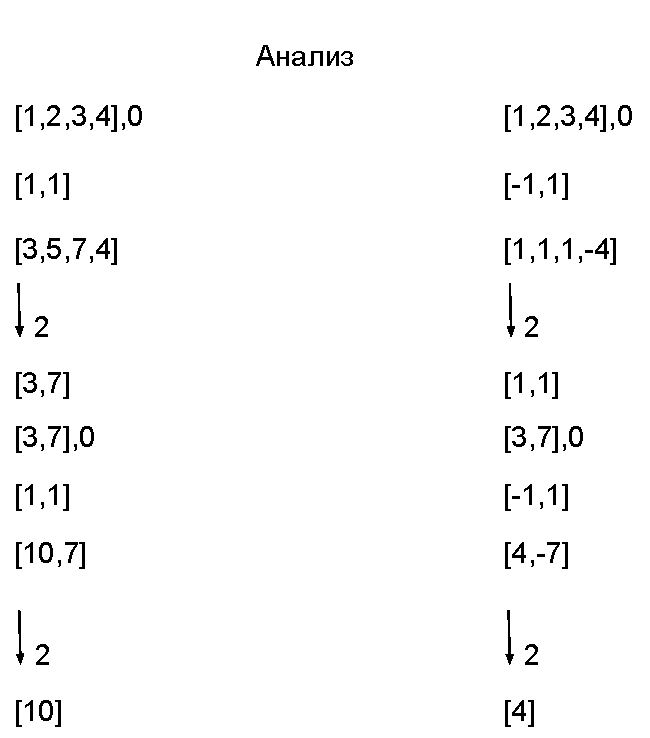
\includegraphics[width=0.4\linewidth]{analyze.pdf}}
\center{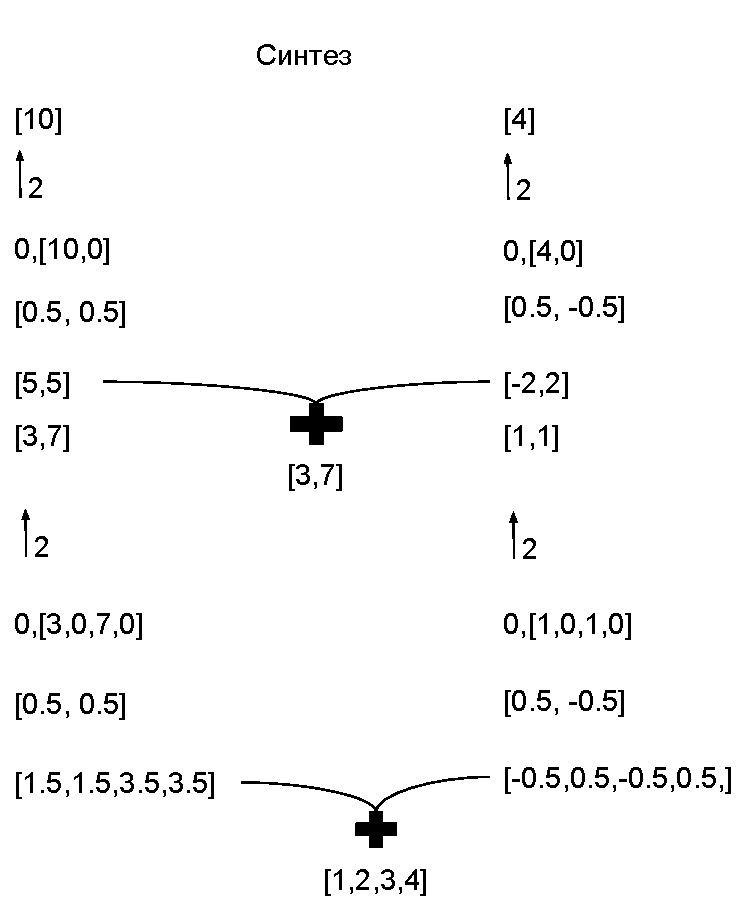
\includegraphics[width=0.4\linewidth]{synthesis.pdf}}
\end{center}


\subsubsection{Двумерное преобразование}
Пусть дана матрица $^{M}\Phi, ^{M}\Phi \in \mathbb{R}^{2^{M}\times2^{M}}$. Применим к каждой строке матрицы один шаг анализа. В результате получим матрицы $_L^{m-1}\Phi$, $_H^{m-1}\Phi$. К каждому столбцу обеих матриц также применим шаг анализа. В итоге получим четыре матрицы $_{LL}^{m-1}\Phi$, $_{LH}^{m-1}\Phi$, $_{HL}^{m-1}\Phi$, $_{HH}^{m-1}\Phi$. $_{LL}^{m-1}\Phi$ - является низкочастотной составляющей двумерного сигнала, остальные три матрицы содержат детализирующую информацию. Таким образом будет выполнен первый шаг двумерного преобразования Хаара. Нужно проделать аналогичные операции с $_{LL}^{m-1}\Phi$ для следующего шага. Такми образом, шаг двумерного преобразования свелся к композиции одномерных преобразований.

Синтез происходит аналогичным образом: в обратном анализу порядке дополняется нулями соответствующая размерность и применяются фильтры Хаара, а затем результаты складываются.

Пусть $^{M}\Phi = _{LL}^{M}\Phi$
\begin{algorithm}[H]
\caption{Алгоритм 2D-анализа}
\begin{algorithmic}
	\For{$k=M \ldots 1$}
		\State $_{LL}^{k-1}\Phi = \downarrow_{2}$ $\{_{LL}^{k}\Phi H_{L}(z_h)H_{L}(z_v)\}$
		\State $_{LH}^{k-1}\Phi = \downarrow_{2}$ $\{_{LL}^{k}\Phi H_{L}(z_h)H_{H}(z_v)\}$
		\State $_{HL}^{k-1}\Phi = \downarrow_{2}$ $\{_{LL}^{k}\Phi H_{H}(z_h)H_{L}(z_v)\}$
		\State $_{HH}^{k-1}\Phi = \downarrow_{2}$ $\{_{LL}^{k}\Phi H_{H}(z_h)H_{H}(z_v)\}$
	\EndFor
\end{algorithmic}
\end{algorithm}
\begin{algorithm}[H]
\caption{Алгоритм 2D-синтеза}
\begin{algorithmic}
	\For{$k=1 \ldots M$}
	\State  $_{LL}^{k-1}\Phi=$ $\uparrow_2$  $\{_{LL}^{k-1}\Phi H_L(z_v^{-1}) + _{LH}^{k-1}\Phi H_L(z_v^{-1})\}H_L(z_h^{-1})+ $ $\uparrow_2$ $\{_{HL}^{k-1}\Phi H_L(z_v^{-1}) + _{HH}^{k-1}\Phi H_L(z_v^{-1})\}H_H(z_h^{-1})$
	\EndFor
\end{algorithmic}
\end{algorithm}	
Полученное $2$-$D$ разложение можно представить в виде диаграммы, где на каждом уровне $LL$, $LH$, $HL$ и $HH$ составляющим соответствуют определенные квадранты. 
\begin{center}
\center{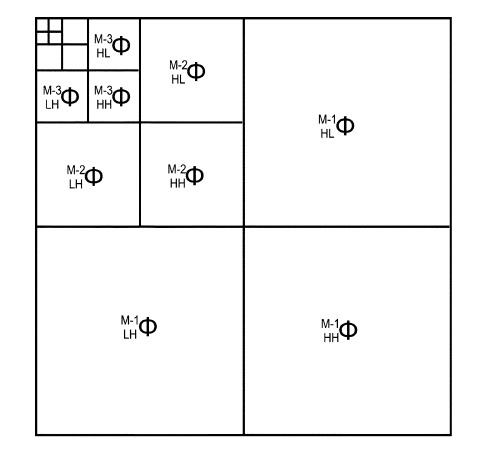
\includegraphics[width=0.6\linewidth]{hwaf_decomp.png}}
\end{center}
\subsubsection{Явные формулы для анализа}
Из алгоритма анализа непосредственно выводятся формулы для $LL$, $LH$, $HL$ и $HH$ составляющих на каждом уровне.
\begin{equation}\label{LL}
_{LL}^{M-m}\Phi=
\downarrow_{2^m} \{^M\Phi\prod\limits_{k = 0}^{m-1} H_L(z_h^{2^k})
							\prod\limits_{k = 0}^{m-1} H_L(z_v^{2^k})\}
\end{equation}
\begin{equation}\label{LH}
_{LH}^{M-m}\Phi=
\downarrow_{2^m} \{^M\Phi H_H(z_v^{2^{m-1}}) \prod\limits_{k = 0}^{m-1} H_L(z_h^{2^k})
							\prod\limits_{k = 0}^{m-2} H_L(z_v^{2^k})\}
\end{equation}
\begin{equation}\label{HL}
_{HL}^{M-m}\Phi=\downarrow_{2^m} \{^M\Phi H_H(z_h^{2^{m-1}}) \prod\limits_{k = 0}^{m-2} H_L(z_h^{2^k})
						\prod\limits_{k = 0}^{m-1} H_L(z_v^{2^k})\}
\end{equation}
\begin{equation}\label{HH}
_{HH}^{M-m}\Phi=\downarrow_{2^m} \{^M\Phi H_H(z_v^{2^{m-1}}) H_H(z_v^{2^{m-1}}) \prod\limits_{k = 0}^{m-2} H_L(z_h^{2^k})
							\prod\limits_{k = 0}^{m-2} H_L(z_v^{2^k})\}
\end{equation}

\subsection{Градиенты. Геометрия Хаджина и Фрайда}
\subsubsection{Геометрия Хаджина и Фрайда}
Вейвлет метод разработан для определенного представления наклонов волнового фронта. Согласно \cite{fourier_1} она называются геометриями Хаджина и Фрайда.
Геометрия Хаджина:
$$_{H}x_{i,j}=-\phi_{i,j}+\phi_{i,j+1}\;;_{H}y_{i,j}=-\phi_{i,j}+\phi_{i+1,j}$$
Получившиеся матрицы $_H^{M}X$, $_H^{M}Y$ имеют размерности $2^M \times(2^M - 1)$ и $(2^M - 1) \times 2^M$ соответственно.
Геометрия Фрайда:
$$_{F}x_{i,j}=\frac{_{H}x_{i,j} + _{H}x_{i+1,j}}{2} = \frac{-\phi_{i,j}+\phi_{i,j+1}-\phi_{i+1,j}+\phi_{i+1,j+1}}{2}$$
$$_{F}y_{i,j}=\frac{_{H}y_{i,j} + _{H}y_{i,j+1}}{2} = \frac{-\phi_{i,j}-\phi_{i,j+1}+\phi_{i+1,j}+\phi_{i+1,j+1}}{2}$$
Получившиеся матрицы $_F^{M}X$, $_F^{M}Y$ имеют одинаковые размерности $2^M - 1 \times 2^M - 1$.


\subsubsection{Градиенты и преобразование Хаара}
Справедливы следующие соотношения.
\begin{equation}\label{_H^MX}
_H^MX = ^M\Phi\sqrt{2}H_H(z_h) 
\end{equation}
\begin{equation}\label{_H^MY}
_H^MY = ^M\Phi\sqrt{2}H_H(z_v)
\end{equation}
\begin{equation}\label{_F^MX}
_F^MX = \frac{_H^MX H_L(z_v)}{\sqrt{2}}=^M\Phi H_H(z_h) H_L(z_v)
\end{equation}
\begin{equation}\label{_F^MY}
_F^MY = \frac{_H^MY H_L(z_h)}{\sqrt{2}}=^M\Phi H_L(z_h) H_H(z_v)
\end{equation}

Можно видеть, что $_H^MX \, _H^MY$ являются производными вперед по $x, \, y$, умноженными на соответствующий шаг $h_{1,2}$ на введенной ранее сетке $\omega_h$. Таким образом исходными данными для метода являются производные вперед $g_1,\,g_2$ по $x,\,y$, , умноженные на соответствующий шаг сетки. В этом случае волновой фронт будет восстановлен с точностью до константы. В случае, если известно среднее арифметическое значений волнового фронта восстановление будет точным.
\subsection{Вывод формул прямого преобразования}
Рассмотрим случай, когда известны вертикальные и горизонтальные наклоны, а также интенсивность волнового фронта. Иначе говоря имеются: $_F^MX$, $_F^MY$, $_H^MX$, $_H^MY$ , $_0^{LL}\Phi$.

Необходимо получить из имеющихся данных получить $2D$-разложение волнового фронта, а затем восстановить сам волновой фронт, применив к полученному разложению стандартный алгоритм синтеза.\cite{new_method1}
Диаграмма разложения которую необходимо получить будет аналогична диаграмме стандартного разложения:
\begin{center}
\center{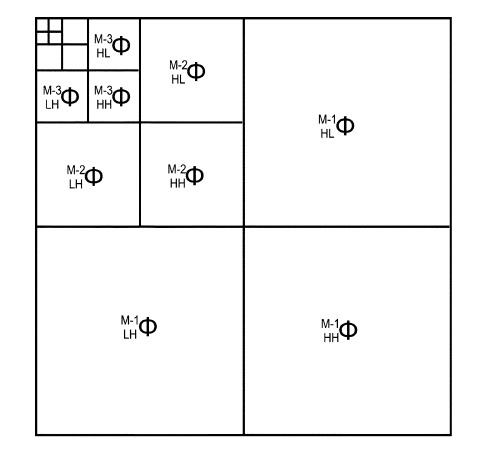
\includegraphics[width=0.6\linewidth]{hwaf_decomp.png}}
\end{center}
Отличаться будут лишь формулы (\ref{LL})-(\ref{HH}). Используя соотношения (\ref{_H^MX})-(\ref{_F^MY}), получим аналоги (\ref{LL})-(\ref{HH}).
\subsubsection{Получение LH, HL квадрантов}
Из соотношений (\ref{_H^MX}), (\ref{_H^MY}) и (\ref{HL}), (\ref{LH}) соответственно, непосредственно вытекает, что:
\begin{center}

$ 	_{HL}^{M-1}\Phi = \downarrow_{2}$ $ _F^MX ;\;_{LH}^{M-1}\Phi = \downarrow_{2}$ $ _F^MY $

\end{center}

Докажем справедливость выражения $H_{H}(z^{2^{m-1}}) = \sqrt{2}^{m-1} H_H(z) \prod \limits_{k=0}^{m-2} H_L(z^{2^k})$
\begin{proof}
Запишем $H_{H}(z^{2^{m-1}})$ в виде полинома
\begin{align*}
&H_{H}(z^{2^{m-1}}) = \frac{1 - z^{2^{m-1}}}{\sqrt{2}} = \frac{(1-z^{2^{m-2}})(1+z^{2^{m-2}})}{\sqrt{2}}=\ldots=\frac{(1-z)(1+z)(1+z^2)\ldots(1+z^{2^{m-2}})}{\sqrt{2}}
\end{align*}
$$H_{H}(z^{2^{m-1}}) = \sqrt{2}^{m-1} H_H(z) \prod \limits_{k=0}^{m-2} H_L(z^{2^k})$$
\end{proof}

\textbf{LH, $m>1$:}
\begin{align*}
&_{LH}^{M-m}\Phi=\downarrow_{2^m} \{^M\Phi [H_H(z_v^{2^{m-1}})] [\prod\limits_{k = 0}^{m-1} H_L(z_h^{2^k})]\prod\limits_{k = 0}^{m-2} H_L(z_v^{2^k})\}=\downarrow_{2^m} \{^M\Phi [\sqrt{2}^{m-1} H_H(z_v) \prod \limits_{k=0}^{m-2} H_L(z_v^{2^k})]
\\&[H_L(z_h)\prod \limits_{k=1}^{m-1} H_L(z_h^{2^k})]\prod\limits_{k = 0}^{m-2} H_L(z_v^{2^k})=\sqrt{2}^{m-1} \downarrow_{2^m} \{^M\Phi H_L(z_h) H_H(z_v)\prod \limits_{k=1}^{m-1} H_L(z_h^{2^k})\prod \limits_{k=0}^{m-2} H_L^2(z_v^{2^k})=
\\&=\sqrt{2}^{m-1} \downarrow_{2^m} \{_F^MY \prod \limits_{k=1}^{m-1} H_L(z_h^{2^k})\prod \limits_{k=0}^{m-2} H_L^2(z_v^{2^k})\}			
\end{align*}
\textbf{HL, $m>1$:}

Выводится аналогично, LH
\[_{HL}^{M-m}\Phi=
\sqrt{2}^{m-1} \downarrow_{2^m} \{_F^MY \prod \limits_{k=0}^{m-2} H_L^{2}(z_h^{2^k})\prod \limits_{k=1}^{m-1} H_L(z_v^{2^k})\}
\]

\subsubsection{Получение HH квадранта}
\textbf{HH, $m=1$:}\cite{new_method2}

Докажем, что $_{HH}^{M-1}\Phi\downarrow_2 \{\frac{\sqrt{2}}{4}[_{H}^MX H_H(z_v) + _{H}^MY H_H(z_h)]\}$
%$_{HH}^{M-1}\Phi = \downarrow_2$ $ [^{M}\Phi H_H(z_h)H_H(z_v)]$
\begin{proof}
Известно, что $_{HH}^{M-1}\Phi = \downarrow_2$ $ [^{M}\Phi H_H(z_h)H_H(z_v)]$.

Распишем \begin{math} _{HH}^{M-1}\Phi = \downarrow_2 \{ \frac{\sqrt{2}}{2}\sqrt{2} ~^{M}\Phi H_H(z_h)H_H(z_v) \} \end{math}, выделив из (\ref{_F^MX}) $_H^MX$ получим:
\[
 _{HH}^{M-1}\Phi = \downarrow_2 \{\frac{\sqrt{2}}{2} ~_{H}^MX H_H(z_v)\} = \downarrow_2 \{\frac{\sqrt{2}}{4}2 ~_{H}^MX H_H(z_v)\}
\]

Разделив (\ref{_F^MX}) на (\ref{_F^MY}) получим:
\[
_{H}^MX H_H(z_v) = _{H}^MY H_H(z_h)
\]
Отсюда получим:
\[
_{HH}^{M-1}\Phi\downarrow_2 \{\frac{\sqrt{2}}{4}[_{H}^MX H_H(z_v) + _{H}^MY H_H(z_h)]
\]
\end{proof}

\textbf{HH, $m>1$:}
\begin{align*}
&_{HH}^{M-m}\Phi=\downarrow_{2^m} \{^M\Phi H_H(z_v^{2^{m-1}}) H_H(z_v^{2^{m-1}}) \prod\limits_{k = 0}^{m-2} H_L(z_h^{2^k})\prod\limits_{k = 0}^{m-2} H_L(z_v^{2^k})\}=
\\&=\downarrow_{2^m} \{^M\Phi \sqrt{2}^{m-1} H_H(z_h) \prod \limits_{k=0}^{m-2} H_L(z_h^{2^k}) \prod \limits_{k=0}^{m-2} H_L(z_h^{2^k}) H_H(z_v^{2^{m-1}})H_L(z_v) \prod \limits _{k=1}^{m-2}H_L(z_v^{2^k})\}=
\\&=\sqrt{2}^{m-1} \downarrow_{2^m} \{_F^MX \prod \limits_{k=0}^{m-2} H_L^2(z_h^{2^k}) H_H(z_v^{2^{m-1}}) \prod \limits_{k=1}^{m-2}H_L(z_v^{2k})    \}
\end{align*}


\subsection{Применение вейвлет метода для восстановления полиномов Цернике}
Под $mse$ и среднеквадратичным отклонением подразумевается:
$$mse = \sqrt{\frac{\sum \limits_{k,l=1}^{n} (X_{kl} - Y_{kl})^2 }{N_1N_2}}$$

$N_1, N_2$ - размерности матриц наклонов. 
%что такое нормировка и супергаусс.

Рассмотрим случай, когда $g_1,\,g_2$ являются разностными производными вперед. В качестве среднего значения $_{LL}^{0}\Phi$ возьмем $1$. Исходный и восстановленный волновые фронты будут нормированы на $1$ и обрезаны супергауссом. В этом случае восстановление будет происходить с точностью до константы.
Выполним восстановление полиномов $Z_3^{-1} = 3\rho^3 - 2\rho  \sin(\phi),\,Z_3^{3} = \rho^3  \cos(3\phi),\,Z_2^{-2} = \rho^2 \sin(2\phi)$ при различных $g_1, g_2$.
\begin{figure}[H]
\center{\includegraphics[width=1\linewidth]{pictures/haar/Z_3^{-1}.png}}
\caption{Полином $Z_3^{-1} = 3\rho^3 - 2\rho \sin(\phi)$, $mse = 7.826969423459203*10^{-19}$.}
\end{figure}

\begin{figure}[H]
\center{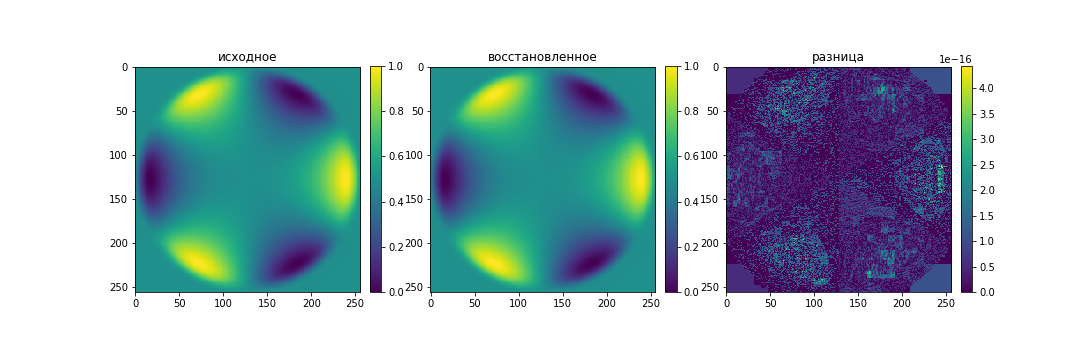
\includegraphics[width=1\linewidth]{pictures/haar/Z_3^3.png}}
\caption{Полином $Z_3^{3} = \rho^3 \cos(3\phi)$, $mse = 2.930551372327761*10^{-19}$.}
\end{figure}

\begin{figure}[H]
\center{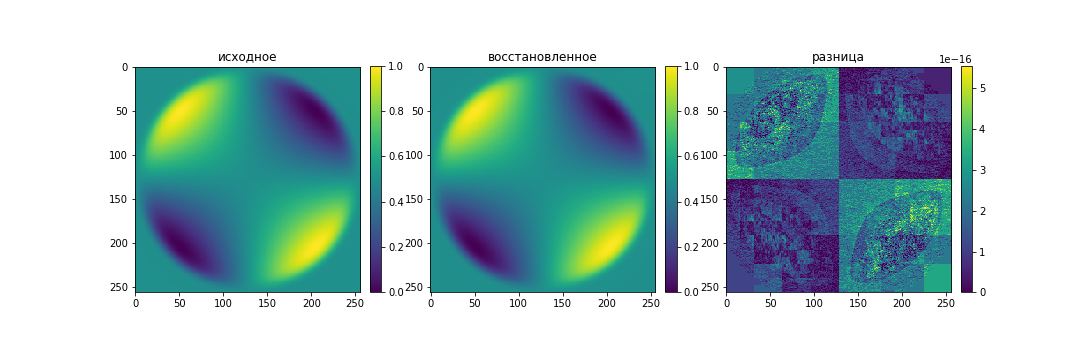
\includegraphics[width=1\linewidth]{pictures/haar/Z_2^-2.png}}
\caption{Полином $Z_2^{-2} = \rho^2 \sin(2\phi)$, $mse = 7.642339638275361*10^{-19}$.}
\end{figure}


\subsection{Работа вейвлет метода при альтернативных $g_1, g_2$}
Видно, что когда $g_1,\, g_2$ являются производными вперед, то восстановление происходит точно. Однако не всегда наклоны имеет такой вид. Рассмотрит работу алгоритма при других $g_1,\, g_2$.

Варианты для $g_1,\,g_2:$
\begin{enumerate} 
\item $g_1 = u_x;\; g_2 = u_y$ - точные значения производных
\item $g_1 = \frac{1}{h_1h_2} \sum \limits_{n=1}^{N_1 - 1} \sum \limits_{m=1}^{N_2 - 1} \int \limits _{\Delta_{nm}} u_\xi(\xi,\eta) d\xi d\eta$ $\overset{\circ}{\varphi}_{nm}(x,y);\;g_2 = \frac{1}{h_1h_2} \sum \limits_{n=1}^{N_1 - 1} \sum \limits_{m=1}^{N_2 - 1} \int \limits _{\Delta_{nm}} u_\eta(\xi,\eta) d\xi d\eta$ $\overset{\circ}{\varphi}_{nm}(x,y)$ 

$$\Delta_{nm} = [x_{n-1}, x_n] \cup [y_{n-1}, y_n] $$
$$\overset{\circ}{\varphi}_{nm}(x,y) = \begin{cases} 1, \, x \in \Delta_{nm} \\ 0, \, else\end{cases}$$

\end{enumerate}

Рассмотрим восстановление полиномов $R_2^2 = \rho^2,\,R_3^3 = \rho^3,\,R_3^1 = 3\rho^3 - 2\rho$ в каждом из вариантов.
\subsubsection{Точные значения производных}
$g_1 = u_x;\; g_2 = u_y$
\begin{figure}[H]
\center{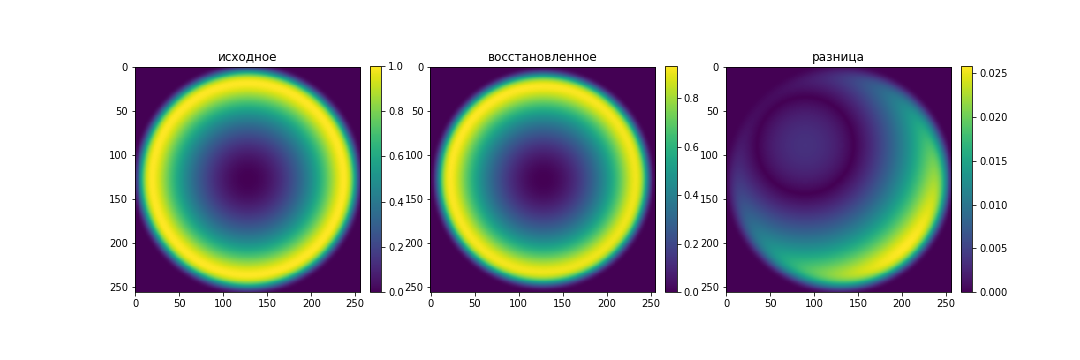
\includegraphics[width=1\linewidth]{pictures/haar/R_2^2_variant1.png}}
\caption{Полином $R_2^2 = \rho^2$, $mse = 3.725633172575012*10^{-5}$.}
\end{figure}

\begin{figure}[H]
\center{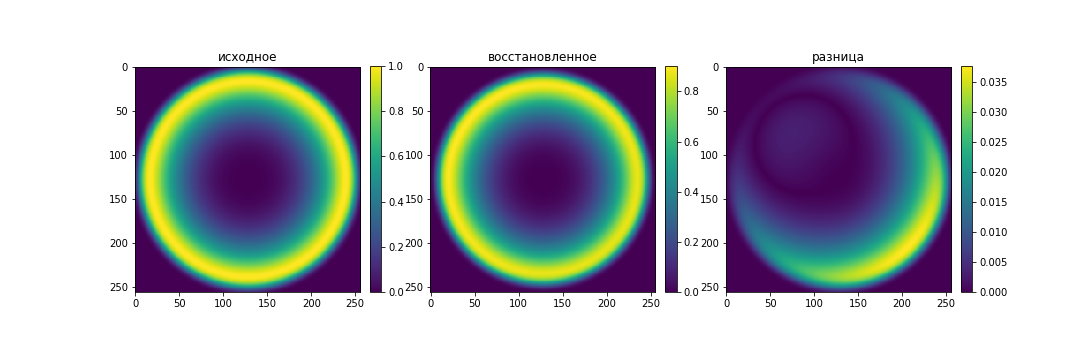
\includegraphics[width=1\linewidth]{pictures/haar/R_3^3_variant1.png}}
\caption{Полином $R_3^3 = \rho^3$, $mse = 4.946969313504892*10^{-5}$.}
\end{figure}

\begin{figure}[H]
\center{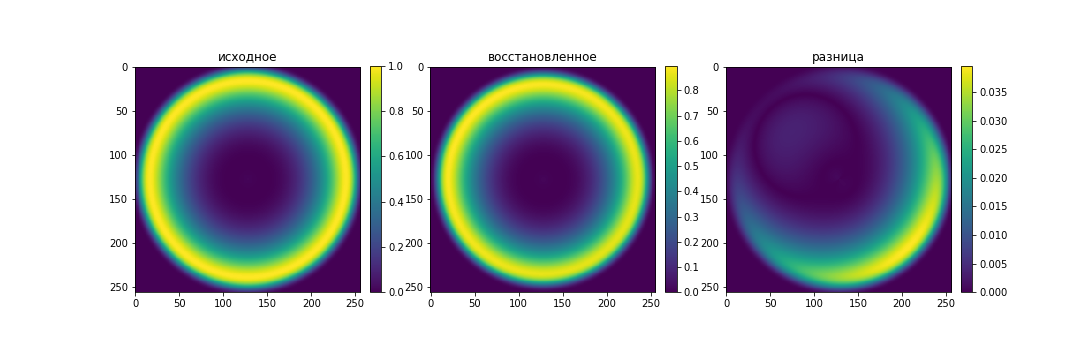
\includegraphics[width=1\linewidth]{pictures/haar/R_3^1_variant1.png}}
\caption{Полином $R_3^1 = 3\rho^3 - 2\rho$, $mse = 5.139470020160782*10^{-5}$.}
\end{figure}

\subsubsection{Случай восстановления по средним локальным апертурам значений наклонов}
$g_1 = \frac{1}{h_1h_2} \sum \limits_{n=1}^{N_1 - 1} \sum \limits_{m=1}^{N_2 - 1} \int \limits _{\Delta_{nm}} u_\xi(\xi,\eta) d\xi d\eta$ $\overset{\circ}{\varphi}_{nm}(x,y);\;g_2 = \frac{1}{h_1h_2} \sum \limits_{n=1}^{N_1 - 1} \sum \limits_{m=1}^{N_2 - 1} \int \limits _{\Delta_{nm}} u_\eta(\xi,\eta) d\xi d\eta$ $\overset{\circ}{\varphi}_{nm}(x,y)$ 

$$\Delta_{nm} = [x_{n-1}, x_n] \cup [y_{n-1}, y_n];\;\;\overset{\circ}{\varphi}_{nm}(x,y) = \begin{cases} 1, \, x \in \Delta_{nm} \\ 0, \, else\end{cases}$$
\begin{figure}[H]
\center{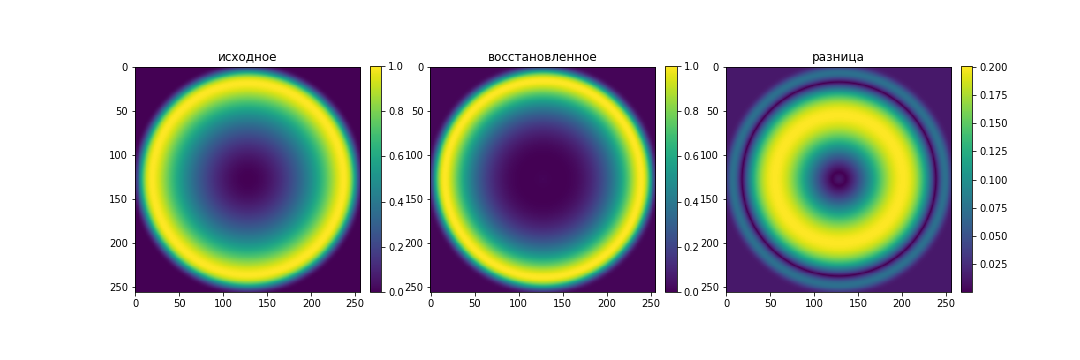
\includegraphics[width=1\linewidth]{pictures/haar/variant2/R_2^2.png}}
\caption{Полином $R_2^2 = \rho^2$, $mse = 0.0004513972414769472$.}
\end{figure}

\begin{figure}[H]
\center{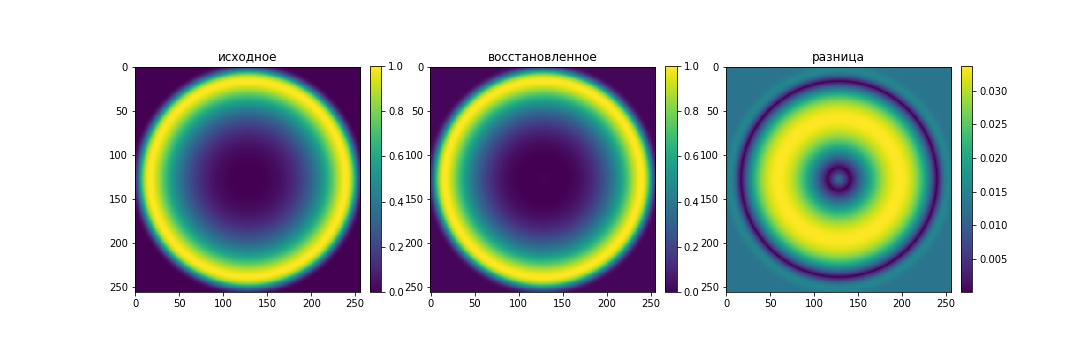
\includegraphics[width=1\linewidth]{pictures/haar/variant2/R_3^3.png}}
\caption{Полином $R_3^3 = \rho^3$, $mse = 8.160988496129328*10^{-5}$.}
\end{figure}

\begin{figure}[H]
\center{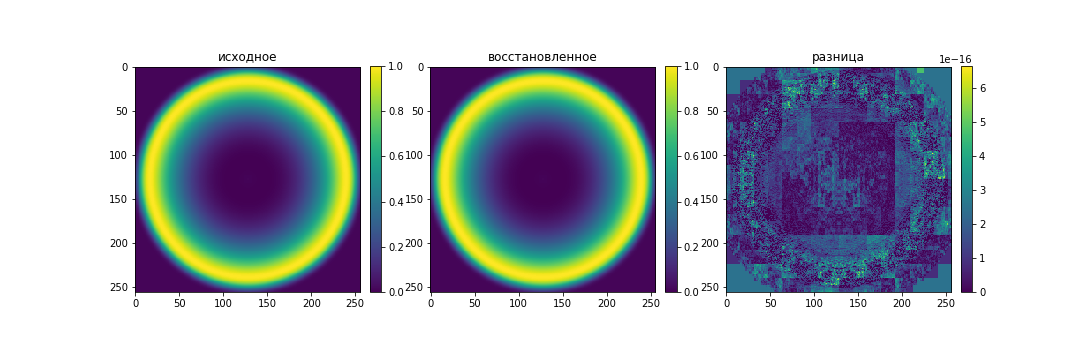
\includegraphics[width=1\linewidth]{pictures/haar/variant2/R_3^1.png}}
\caption{Полином $R_3^1 = 3\rho^3 - 2\rho$, $mse = 6.515915893131193*10^{-19}$.}
\end{figure}

\subsubsection{Погрешность восстановления}
Вейвлет метод восстанавливает значения волнового фронта точно, в том случае, когда $g_1,\, g_2$ являются первыми разностными производными. В противном случае существует погрешность восстановления. (Предполагается, что $f \in C^1$).
$$\frac{f(x+h)-f(x)}{h} = f'(x) + O(h)$$
$$f'(x) = \frac{f(x+h)-f(x)}{h} + O(h)$$
\section{Вариационный метод восстановления волнового фронта}

Рассмотрим функционал $$J(u) = \int \limits_0^{2\pi} \int \limits_0^{2\pi} ((u_x - g_1)^2 + (u_y-g_2)^2 + \alpha u^2 )dxdy$$
Функция $u$ принадлежит соболевскому пространству $W_{2\pi}^{1}(\Omega)$, пространству периодических функций, определенных в области $\Omega = [0,\,2\pi]  \times [0,\,2\pi]$ и имеющих суммируемые с квадратом первые обобщенные производные по $x,\,y$. Минимизация функционала позволяет найти функцию $u$ с наименьшими квадратичными отклонениями градиента от измеренных локальных наклонах $g_1,\, g_2$. Дополнительное слагаемое $\alpha u^2$ , является регуляризатором Тихонова с параметром $\alpha$. Благодаря регуляризатору устраняются проблемы единственности минимума функционала и возможной погрешности исходных данных. Необходимым условием минимума функционала является:
\begin{equation}\label{nessasary condition}
(u_x, \phi_x) + (u_y,\phi_y) + \alpha(u, \phi) = (g_1, \phi_x) + (g_2, \phi_y),\;\;\forall\phi \in W_{2\pi}^{1}(\Omega)
\end{equation}
Здесь $(\cdot\,,\cdot)$ - скалярное произведение в $L_2(\Omega)$.
\subsection{Проекционно-разностная схема}
На $\Omega$ введем сетку $\omega_h = \{(x_i, y_j) \,:\, x_i = ih_1,\,y_j = jh_2,\, i = 0..N_1,\, j = 0..N_2;\; h_{1,2}N_{1,2} = 2\pi\}$. Определим на $\Omega$ систему финитных базисных функций $\{\phi_i(x)\} ,\, i \in [0,\,N-1]$.
$$
\phi_i(x) = 
 \begin{cases}
  \frac{x-x_{i-1}}{h} , x \in [x_{i-1},x_i] \\ 
   \frac{x_{i+1} - x}{h}, x \in [x_{i},x_{i+1}]   \\
   0 \notin [x_{i-1},x_{i+1}].
 \end{cases} i \in [1, N-1];\;\;\;
\phi_0(x) = 
 \begin{cases}
  \frac{x_1-x}{h} , x \in [x_{0},x_1] \\ 
   \frac{x - x_{N-1}}{h}, x \in [x_{N-1},x_{N}]   \\
   0 \in [x_{1},x_{N-1}].
 \end{cases}
$$

Введем пространство конечных элементов $W_h = \mathscr{L}\{\phi_i(x)\phi_j(y)\}_{i,j=0}^{N_1 - 1,N_2-1} \in W_{2\pi}^{1}(\Omega)$. Проекционная схема решения $\ref{nessasary condition}$ состоит в нахождении функции $u^h \subset W_h$, которая при любых $k,\,l$ удовлетворяет тожеству:
\begin{equation}\label{mult diff scheme}
(u_x^h,\phi_x)+(u_y^h,\phi_y) + \alpha(u^h,\phi) = (g^1,\phi_x) + (g^2,\phi_y)
\end{equation}
Где:
$$\phi(x,y) = \phi_k(x)\phi_l(y)$$
$$u^h(x,y) = \sum \limits_{i=0}^{N_1-1} \sum \limits_{j=0}^{N_2-1} u_{ij}\phi_i(x)\phi_j(y)$$
$$u_{ij} = u(x_i,y_i)$$

Подставив в (\ref{mult diff scheme}) необходимые значения получим разностную схему \cite{marchuck}, \cite{vatiational_base}

\begin{equation}
B_2 \Lambda_1 u + B_1 \Lambda_2 u + \alpha B_1 B_2 u = F(g_1,g_2)
\end{equation}
Правая часть $F(g_1,g_2)$ не определена однозначно и будет уникальной для каждого представления $g_1,\,g_2$.
Введем дополнительный регуляризатор $\gamma\Lambda_1\Lambda_2u$. В таком случае схема будет иметь вид:
\begin{equation}\label{scheme}
B_2 \Lambda_1 u + B_1 \Lambda_2 u + \alpha B_1 B_2 u + \gamma\Lambda_1\Lambda_2u = F(g_1,g_2)
\end{equation}
Разделим обе части равенства на $h_1h_2$. Это необходимо будет участь в дальнейшем при получении $F$.
В этом случае операторы $\Lambda_{1,2},\,B_{1,2}$ в матричной форме имеют вид:
$$\Lambda_i = \frac{1}{h_i^2}
\begin{bmatrix}
2 & -1 & 0 & \ldots & 0 & 0 & -1\\
-1 & 2 & -1 & \ldots & 0 & 0 & 0\\
0 & -1 & 2 & \ldots &0 & 0 & 0\\
\ldots & \ldots & \ldots & \ldots & \ldots & \ldots & \ldots &\\
0 & 0 & 0 & \ldots & -1 & 2 & -1\\
-1 & 0 & 0 & \ldots & 0 & -1 & 2
\end{bmatrix}
$$
$$
\qquad B_i = 
\begin{bmatrix}
\frac{2}{3} & \frac{1}{6} & 0 & \ldots & 0 & 0 & \frac{1}{6}\\
\frac{1}{6} & \frac{2}{3} & \frac{1}{6} & \ldots & 0 & 0 & 0\\
0 & \frac{1}{6} & \frac{2}{3} & \ldots &0 & 0 & 0\\
\ldots & \ldots & \ldots & \ldots & \ldots & \ldots & \ldots &\\
0 & 0 & 0 & \ldots & \frac{1}{6} & \frac{2}{3} & \frac{1}{6}\\
\frac{1}{6} & 0 & 0 & \ldots & 0 & \frac{1}{6} & \frac{2}{3} \\
\end{bmatrix} = E - \frac{h_i^2}{6}\Lambda_i$$
Благодаря делению на $h_1h_2\;\Lambda$ является оператором второй разностной производной.
Воспользуемся методом Фурье для решения разностной схемы. Будем искать собственные функции оператора $\Lambda$ в виде:
$$v_k = e^{ikx}$$
Напомним решение задачи Штурма-Лиувилля в $H_h$ для оператора второй разностной производной:
$$\begin{cases}
y_{\overline{x}x} + \lambda y_i = 0,\quad i = \overline{1\ldots N-1} \\
y_0 = y_N
\end{cases}$$
Подставив в уравнение получим собственные значения 
$$
\lambda_k = \frac{4}{h^2} \sin^2(\frac{kh}{2}),\quad k = \overline{0 \ldots N-1}
$$
Так как $B = E - \frac{h_i^2}{6}\Lambda_i$, то собственными значениями оператора B будут:
$$
\mu_k = 1 - \frac{h^2}{6}\lambda_k,\quad k = \overline{0 \ldots N-1}
$$

Будем искать решение в виде разложения по собственным функциям:
$$u_{ij} = \sum \limits_{k=0}^{N_1 - 1} \sum \limits_{l=0}^{N_2 - 1} \overline{u}_{kl}v_k(x_i)v_l(y_j)$$
Подставив в разностное уравнение наше решение, и используя линейную независимость собственных функций, получим:
$$\mu_l \lambda_k + \mu_k \lambda_l + \alpha \mu_k \mu_l + \gamma \lambda_k \lambda_l = f_{kl}$$
Где $f_{kl}$ - преобразование Фурье $F(g_1,g_2)$.
Таким образом:
$$u_{kl} = \frac{f_{kl}}{\mu_l \lambda_k + \mu_k \lambda_l + \alpha \mu_k \mu_l + \gamma \lambda_k \lambda_l}$$
\subsection{Различные представления правой части}
Как было отмечено выше вид $g_1,\,g_2$ определен неоднозначно. Рассмотрим несколько вариантов представления $g_1, g_2$ и получим для каждого $F(g_1,g_2)$.
\begin{enumerate}
\item$g_{1,2}(x,y) = \sum \limits_{i=0}^{N_1-1} \sum \limits_{j=0}^{N_2-1}g_{1,2}^{ij}\phi_i(x)\phi_j(y),\, g_{ij} = g(x_i,y_j)$
\item$g_1 = \frac{1}{h_1h_2} \sum \limits_{n=1}^{N_1 - 1} \sum \limits_{m=1}^{N_2 - 1} \int \limits _{\Delta_{nm}} u_\xi(\xi,\eta) d\xi d\eta$ $\overset{\circ}{\varphi}_{nm}(x,y)$

$g_2 = \frac{1}{h_1h_2} \sum \limits_{n=1}^{N_1 - 1} \sum \limits_{m=1}^{N_2 - 1} \int \limits _{\Delta_{nm}} u_\eta(\xi,\eta) d\xi d\eta$ $\overset{\circ}{\varphi}_{nm}(x,y)$ 

Здесь
$$\Delta_{nm} = [x_{n-1}, x_n] \cup [y_{n-1}, y_n] $$
$$\overset{\circ}{\varphi}_{nm}(x,y) = \begin{cases} 1, \, x \in \Delta_{nm} \\ 0, \, else\end{cases}$$ 
\end{enumerate}
Учитывая то, что правая часть в (\ref{scheme}) была нормирована на $h_1h_2$
\begin{equation}\label{F}
F = \frac{1}{h_1h_2}((g_1,\phi_x) + (g_2,\phi_y))
\end{equation} 
\subsubsection{Разложение точных значений производных по базисным функциям $W_h$}
$$g_{1,2}(x,y) = \sum \limits_{i=0}^{N_1-1} \sum \limits_{j=0}^{N_2-1}g_{1,2}^{ij}\phi_i(x)\phi_j(y),\, g_{ij} = g(x_i,y_j)$$
$$g_{1,2}(x,y) = \sum \limits_{i=0}^{N_1-1} \sum \limits_{j=0}^{N_2-1}g_{1,2}^{ij}\phi_i(x)\phi_j(y),\, g_{ij} = g(x_i,y_j)$$
Найдем $F(g_1,g_2)$. 
Пусть $F_1 = \frac{1}{h_1h_2}(g_1,\phi_x),\, F_2 = \frac{1}{h_1h_2}(g_2, \phi_y)$.

\begin{align*}
&F_1 = (g_1, \phi_x) = \sum \limits_{n = 0}^{N_1 - 1} \sum \limits_{m = 0}^{N_2 - 1} \int \limits_0^{2\pi}\int \limits_0^{2\pi} g_1^{nm}\phi_n(x)\phi_m(y) \phi'_k(x) \phi_l(y) dx dy =\\& 
\sum \limits_{n = 0}^{N_1 - 1} \sum \limits_{m = 0}^{N_2 - 1} g_1^{nm} \int \limits_0^{2\pi} \phi_n(x) \phi'_k(x) dx \int \limits_0^{2\pi} \phi_m(y) \phi_l(y) dy
\end{align*}

$\int \limits_0^{2\pi} \phi_n(x) \phi'_k(x) dx  = G_{kn} =
\begin{cases} 
    0, \, k = n \\ 
    -1, \, k - n = -1 \\
    1, \, n - k = 1 \\
    0, else
\end{cases}
\int \limits_0^{2\pi} \phi_m(y) \phi_l(y) dy = B_{ml} =
\begin{cases}
    \frac{2}{3}, \, m = l \\
    \frac{1}{6}, \mid m-l \mid = 1\\
    0, else
\end{cases}$

$(g_1, \phi_x) = \sum \limits_{n = 0}^{N_1 - 1} \sum \limits_{m = 0}^{N_2 - 1} g_1^{nm} G_{kn} B_{ml} = 
\sum \limits_{n = 0}^{N_1 - 1} \big(\sum \limits_{m = 0}^{N_2 - 1} G_{kn} g_1^{nm} \big) B_{ml} = G_1 g_1 B_2
$

Аналогично получаем, что $F_2 = B_1 g_2 G_2$.
Таким образом $F = G_1 g_1 B_2 + B_1 g_2 G_2$.
Матрицы $G_1,\,G_2$ имеют следующий вид:
$$G_1 = \frac{1}{2h_1}
\begin{bmatrix}
0 & -1 & 0 & \ldots & 0 & 0 & 1\\
1 & 0 & 1 & \ldots & 0 & 0 & 0\\
0 & 1 & 0 & \ldots &0 & 0 & 0\\
\ldots & \ldots & \ldots & \ldots & \ldots & \ldots & \ldots &\\
0 & 0 & 0 & \ldots & 1 & 0 & -1\\
-1 & 0 & 0 & \ldots & 0 & 1 & 0
\end{bmatrix}
$$
$$G_2 = \frac{1}{2h_2}
\begin{bmatrix}
0 & 1 & 0 & \ldots & 0 & 0 & -1\\
-1 & 0 & 1 & \ldots & 0 & 0 & 0\\
0 & -1 & 0 & \ldots &0 & 0 & 0\\
\ldots & \ldots & \ldots & \ldots & \ldots & \ldots & \ldots &\\
0 & 0 & 0 & \ldots & -1 & 0 & 1\\
1 & 0 & 0 & \ldots & 0 & -1 & 0
\end{bmatrix}
$$

$$G_2 = \frac{h_1}{h_2} G_1^T$$

\subsubsection{Случай восстановления по средним локальным апертурам значений наклонов}
\begin{equation}\label{g_1}
g_1 = \frac{1}{h_1h_2} \sum \limits_{n=1}^{N_1 - 1} \sum \limits_{m=1}^{N_2 - 1} \int \limits _{\Delta_{nm}} u_\xi(\xi,\eta) d\xi d\eta \,\overset{\circ}{\varphi}_{nm}(x,y)
\end{equation}
\begin{equation}\label{g_2}
g_2 = \frac{1}{h_1h_2} \sum \limits_{n=1}^{N_1 - 1} \sum \limits_{m=1}^{N_2 - 1} \int \limits _{\Delta_{nm}} u_\eta(\xi,\eta) d\xi d\eta \, \overset{\circ}{\varphi}_{nm}(x,y)
\end{equation}

Здесь
$$\Delta_{nm} = [x_{n-1}, x_n] \cup [y_{n-1}, y_n]; \;\;\overset{\circ}{\varphi}_{nm}(x,y) = \begin{cases} 1, \, (x,\,y) \in \Delta_{nm} \\ 0, \, else\end{cases}$$
%Пусть $F_1 = (g_1,\phi_x),\, F_2 = (g_2, \phi_y)$. Найдем $F_1$. 
Покажем, что $g_1,\, g_2$ действительно аппроксимируют производные. Предположим, что $u$ непрерывна и дифференцируема на $W$. Тогда справедливо следующее:
\begin{align*}
&g_1 = \frac{1}{h_1h_2} \sum \limits_{n=1}^{N_1 - 1} \sum \limits_{m=1}^{N_2 - 1} \int \limits _{\Delta_{nm}} u_\xi(\xi,\eta) d\xi d\eta \, \overset{\circ}{\varphi}_{nm}(x,y) = 
\frac{1}{h_1h_2} \sum \limits_{n=1}^{N_1 - 1} \sum \limits_{m=1}^{N_2 - 1} \int \limits _{y_{m-1}}^{y_m}  d\eta \int \limits_{x_{n-1}}^{x_n} u_\xi(\xi,\eta) d\xi \, \overset{\circ}{\varphi}_{nm}(x,y) =\\&  
\frac{1}{h_1h_2} \sum \limits_{n=1}^{N_1 - 1} \sum \limits_{m=1}^{N_2 - 1} \int \limits _{y_{m-1}}^{y_m} u(x_n,\eta) - u(x_{n-1}, \eta) d\eta\, \overset{\circ}{\varphi}_{nm}(x,y) = \{\text{теорема Лагранжа};\psi_n \in [x_{n-1}, x_n] \} \\&=
\frac{1}{h_1h_2} \sum \limits_{n=1}^{N_1 - 1} \sum \limits_{m=1}^{N_2 - 1} \int \limits _{y_{m-1}}^{y_m} u'_x(\psi_n,\eta)h_1 d\eta\, \overset{\circ}{\varphi}_{nm}(x,y) = \{ \text{первая теорема о среднем}; \zeta_m \in [y_{m-1}, y_m] \} \\&= 
\frac{1}{h_1h_2} \sum \limits_{n=1}^{N_1 - 1} \sum \limits_{m=1}^{N_2 - 1} u'_x(\psi_n,\zeta_m)h_1 h_2, \overset{\circ}{\varphi}_{nm}(x,y) = 
\sum \limits_{n=1}^{N_1 - 1} \sum \limits_{m=1}^{N_2 - 1} u'_x(\psi_n,\zeta_m) \, \overset{\circ}{\varphi}_{nm}(x,y)
\end{align*}
Аналогично:
$g_2 = \sum \limits_{n=1}^{N_1 - 1} \sum \limits_{m=1}^{N_2 - 1} u'_y(\psi_n,\zeta_m) \, \overset{\circ}{\varphi}_{nm}(x,y), \;\;(\psi_n, \zeta_m) \in \Delta_{nm}$.

Найдем $F(g_1,g_2)$. 

Пусть $F_1 = (g_1,\phi_x),\, F_2 = (g_2, \phi_y)$. 

Найдем $F_1$.
Заменим в (\ref{g_1}) $\frac{1}{h_1h_2}\int \limits _{\Delta_{nm}} u_\xi(\xi,\eta) d\xi d\eta$ на $g_1^{nm}$, тогда:
\begin{align*}
&F_1 = (g_1,\phi_x) = \int \limits_0^{2\pi} \int \limits_0^{2\pi} \sum \limits_{n=1}^{N_1-1} \sum \limits_{m=1}^{N_2-1} g_1^{nm} \overset{\circ}{\varphi}_{nm}(x,y) \phi'_s(x) \phi_t(y) dxdy  = 
\int \limits_0^{2\pi} \int \limits_0^{2\pi} g_1^{st}  \overset{\circ}{\varphi}_s(x)\overset{\circ}{\varphi}_t(y)\phi'_s(x)\phi_t(y)dxdy +\\&
\int \limits_0^{2\pi} \int \limits_0^{2\pi} g_1^{s+1,t}  \overset{\circ}{\varphi}_{s+1}(x)\overset{\circ}{\varphi}_t(y)\phi'_s(x)\phi_t(y)dxdy +
\int \limits_0^{2\pi} \int \limits_0^{2\pi} g_1^{s,t+1}  \overset{\circ}{\varphi}_s(x)\overset{\circ}{\varphi}_{t+1}(y)\phi'_s(x)\phi_t(y)dxdy +\\&
\int \limits_0^{2\pi} \int \limits_0^{2\pi} g_1^{s+1,t+1}  \overset{\circ}{\varphi}_s(x)\overset{\circ}{\varphi}_t(y)\phi'_{s+1}(x)\phi_{t+1}(y)dxdy = \frac{(g_1^{st} - g_1^{s+1,t} + g_1^{s,t+1} - g_1^{s+1,t+1})h_2}{2}
\end{align*}

Аналогично:

\begin{math}
F_2 = (g_2, \phi_y) = \frac{(g_2^{st} - g_2^{s,t+1} + g_2^{s+1,t} - g_2^{s+1, t+1})h_1}{2}
\end{math}

В итоге:
\begin{equation}
F = \frac{g_1^{st} - g_1^{s+1,t} + g_1^{s,t+1} - g_1^{s+1,t+1}}{2h_1} + \frac{g_2^{st} - g_2^{s,t+1} + g_2^{s+1,t} - g_2^{s+1, t+1}}{2h_2}
\end{equation}
\subsection{Получение частотных характеристик для различных представлений правой части}
Для исследования описанного метода восстановления наиболее информативно будет изучить влияние данного оператора на спектры входных и выходных данных. Для этого следует ввести понятие частотной характеристики. Частотная характеристика - это зависимость амплитуды выходного сигнала некоторой системы от частоты её входного гармонического сигнала. То есть значение частотной характеристики при некоторой частоте указывает, во сколько раз амплитуда сигнала на выходе системы отличается от амплитуды входного сигнала на этой же частоте. Данная характеристика показывает наиболее общую картину о свойствах некоторых операторов или передаточных функций. В данном разделе будет проведено исследование частотной характеристики вариационного метода при различных $g_1,\,g_2$ для получения большей информации о его эффективности. Это даст наиболее полное представление о достоинствах и недостатках метода восстановления. Для исследования частотной характеристики данного метода рассмотрим необходимое условие минимума функционала:
\begin{equation}\label{scheme2}
B_2 \Lambda_1 u + B_1 \Lambda_2 u + \alpha B_1 B_2 u + \gamma \Lambda_1 \Lambda_2 u = B_1 G_1 g_1 + G_2 B_2 g_2
\end{equation}
\subsubsection{Точные значения производных}
Пусть точное решение $v(x,y) = e^{ikx}e^{ily}, k \neq 0, l \neq 0$

$g_1 = v_x =ixe^{ikx}e^{ily},\, g_2 = v_y = ile^{ikx}e^{ily}$

Произведя соответствующие вычисления получаем:

$$(g_1, \phi_x) = h \lambda_k e^{ikx_n} \frac{h}{l^2} \lambda_l e^{ily_m}$$

$$(g_2, \phi_y) = h \lambda_l e^{ily_m} \frac{h}{k^2} \lambda_k e^{ikx_n}$$

Теперь рассмотрим приближенное решение $u(x,y) = u_{kl} e^{ikx}e^{ily}$
Подставим ее в левую часть тождества. Использовав собственные значения
операторов $B_{1,2} ,\,\Lambda_{1,2}$ , получим:
\begin{equation}
(\mu_l \lambda_k + \mu_k \lambda_l + \alpha \mu_k \mu_l + \gamma \lambda_k \lambda_l)e^{ikx}e^{ily} = (\frac{1}{k^2} + \frac{1}{l^2})\lambda_k\lambda_lu_{kl}e^{ikx}e^{ily}
\end{equation}
Получаем частотную характеристику
\begin{equation}
H_{kl} = \frac{1}{u_{kl}} = \frac{(\frac{1}{k^2} + \frac{1}{l^2})\lambda_k\lambda_l}{\mu_l \lambda_k + \mu_k \lambda_l + \alpha \mu_k \mu_l + \gamma \lambda_k \lambda_l}
\end{equation}
Не ограничивая общности положим $h_1 = h_2 = h$. Используем замену $\omega_k = kh, \omega_l = lh$. Получим:
\begin{equation}
H_{kl} = \frac{12 \sin^2\frac{\omega_k}{2}  \sin^2\frac{\omega_l}{2}(\frac{1}{\omega_k^2} + \frac{1}{\omega_l^2}) }
            { \sin^2\frac{\omega_k}{2}(2 +  \cos\omega_l) +  \sin^2\frac{\omega_l}{2}(2  +  \cos\omega_k) + \frac{\alpha h^2}{12}(2 +  \cos\omega_k)(2 +  \cos\omega_l) + 12\gamma \, \sin^2\frac{\omega_k}{2}  \sin^2\frac{\omega_l}{2}}
\end{equation}
На рис. \ref{ris:cont_plt} изображена частотная характеристика $H=\{H_{kl}\}^{\frac{N}{2}}_{k,\,l=-\frac{N}{2}}$ с нормированными координатами $f_k = \frac{\omega_k}{2\pi} ,\, f_l = \frac{\omega_l}{2\pi}$. $\alpha = 0.00001\,,\gamma = 0.1$
\begin{figure}[H]
\center{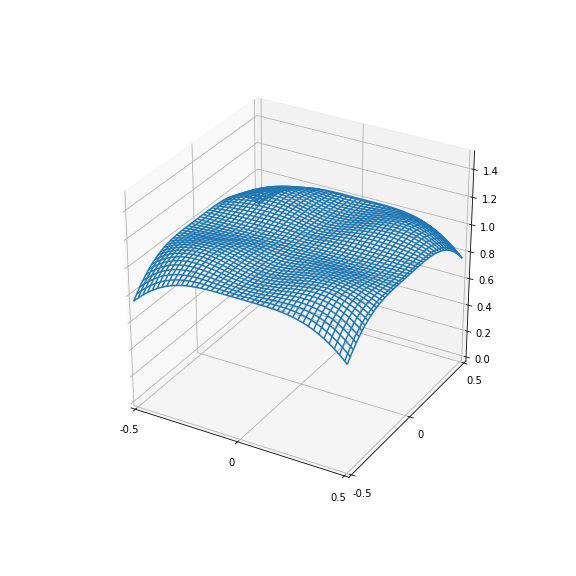
\includegraphics[width=0.8\linewidth]{pictures/variational/freq_char/3dcont.png}}
\caption{Частотная характеристика при точных значениях производных. $\alpha = 0.00001\,,\gamma = 0.1$.}
\label{ris:cont_plt}
\end{figure}
\begin{figure}[H]
\center{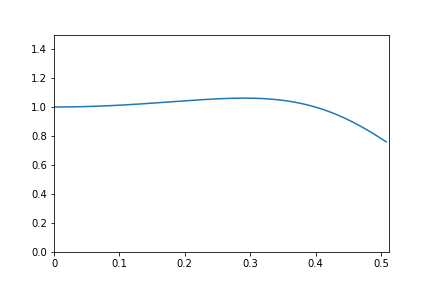
\includegraphics[width=0.6\linewidth]{pictures/variational/freq_char/2dcont.png}}
\caption{Частотная $H_{ll}$ характеристика при точных значениях производных при $\alpha = 0.00001\,,\gamma = 0.1$}
%\label{ris:cont_plt}
\end{figure}

Ниже приведена частотная характеристика $H_{ll}$ при $\alpha = 0.00001$ и различных $\gamma$.
\begin{figure}[H]
\center{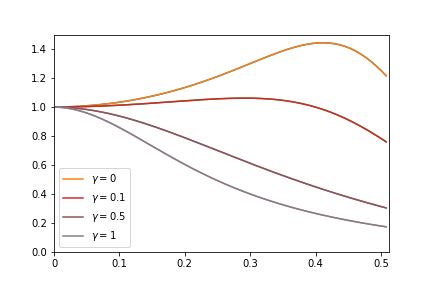
\includegraphics[width=0.6\linewidth]{pictures/variational/freq_char/2dcont4vars.png}}
\caption{Частотная характеристика $H_{ll}$ при $\alpha = 0.00001$ и различных $\gamma$.}
\end{figure}
\subsubsection{Случай восстановления по средним локальным апертурам значений наклонов}
В этом случае:
$$g_1(x,y) = \frac{1}{h_1h_2} \sum \limits_{n=1}^{N_1 - 1} \sum \limits_{m=1}^{N_2 - 1} \int \limits _{\Delta_{nm}} u_\xi(\xi,\eta) d\xi d\eta \, \overset{\circ}{\varphi}_{nm}(x,y)$$

$$g_2(x,y) = \frac{1}{h_1h_2} \sum \limits_{n=1}^{N_1 - 1} \sum \limits_{m=1}^{N_2 - 1} \int \limits _{\Delta_{nm}} u_\eta(\xi,\eta) d\xi d\eta \, \overset{\circ}{\varphi}_{nm}(x,y)$$
$$\Delta_{nm} = [x_{n-1}, x_n] \cup [y_{n-1}, y_n];\;\;\overset{\circ}{\varphi}_{nm}(x,y) = \begin{cases} 1, \, x \in \Delta_{nm} \\ 0, \, else\end{cases}$$

Пусть точное решение $$v(x,y) = e^{ikx}e^{ily}, k \neq 0, l \neq 0$$
Учитывая что, $F$ в этом случае выглядит так:
$$F = \frac{g_1^{st} - g_1^{s+1,t} + g_1^{s,t+1} - g_1^{s+1,t+1}}{2h_1} + \frac{g_2^{st} - g_2^{s,t+1} + g_2^{s+1,t} - g_2^{s+1, t+1}}{2h_2}$$
\begin{equation} \label{g_1}
g_1^{nm} = \frac{1}{h_1h_2}\int \limits _{\Delta_{nm}} u_\xi(\xi,\eta) d\xi d\eta
\end{equation}
\begin{equation}
g_2^{nm} = \frac{1}{h_1h_2}\int \limits _{\Delta_{nm}} u_\eta(\xi,\eta) d\xi d\eta
\end{equation}

Если $v_x(x,y) = ike^{ikx}e^{ily}$, то:
\begin{align*}
&g_1^{nm} = \frac{1}{h_1h_2} \int \limits _{\Delta_{nm}} u_\xi(\xi,\eta) d\xi d\eta = \frac{1}{h_1h_2} \int \limits _{\Delta_{nm}} ike^{ik\xi}e^{il\eta} d\xi d\eta = 
\frac{ik}{h_1 h_2} \int \limits_{x_{n-1}}^{x_n}e^{ik\xi}d\xi \int \limits_{y_{m-1}}^{y_m} e^{il\eta}d\eta = \\& \frac{e^{ikx_{n-1}} e ^{ily_{m-1}}(e^{ikh_1} - 1)(e^{ilh_2} - 1)}{h_1 h_2 il}
\end{align*}
Учитывая, что $(g_1, \phi_x) = F_1 = \frac{(g_1^{st} - g_1^{s+1,t} + g_1^{s,t+1} - g_1^{s+1,t+1})h_2}{2} $, получаем:
\begin{align*}
&(g_1, \phi_x) = \frac{(e^{ikh_1}-1)(e^{ilh_2} - 1)(e^{ikx_{s-1}}e^{ily_{t-1}} - 
e^{ikx_s}e^{ily_{t-1}} + e^{ikx_{s-1}}e^{ily_t} - e^{ikx_s}e^{ily_t})}{2ilh_1} = 
\\& = \frac{(e^{ikh_1}-1)(e^{ilh_2} - 1)e^{ikx_{s-1}}e^{ily_{t-1}}(1 - e^{ikh_1} + e^{ilh_2} - e^{ikh_1}e^{ilh_2})}{2ilh_1} = \\& = \frac{(e^{ikh_1}-1)(e^{ilh_2} - 1)e^{ikx_{s-1}}e^{ily_{t-1}}(1-e^{ikh_1})(1+e^{ilh_2})}{2ilh_1} = 
\frac{e^{ikx_{s-1}}e^{ily_{t-1}} (1-e^{ikh_1})^2(1-e^{2ilh_2})}{2ilh_1}
\end{align*}

Далее, учитывая что $(e^{-ikh_1} - 2 + e^{ikh_1}) = -4\sin^2(\frac{kh_1}{2}) = \lambda_k h_1^2$ и $\frac{e^{-ilh_2} - e^{ikh_2}}{2i} = -\sin (lh_2)$, получим:
\begin{align*}
\frac{e^{ikx_s}e^{ily_t}(e^{-ikh_1}-2+e^{ikh_1})e^{ily_t}(e^{-ilh_2}-e^{ilh_2})}{2lh_1i} = \frac{e^{ikx_s}e^{ily_t}h_1\lambda_k\sin(lh_2)}{l}
\end{align*}
Не ограничивая общности положим $h_1 = h_2 = h$. Используем замену $\omega_k = kh, \omega_l = lh$.
$$(g_1, \phi_x) = \frac{4}{\omega_l h^2}  \sin^2\frac{\omega_k}{2}  \sin\,\omega_l e^{ikx_n}e^{ily_m}$$
Аналогично находится $(g_2, \phi_y)$.
$$(g_2, \phi_y) = \frac{4}{\omega_k h^2}  \sin^2\frac{\omega_l}{2}  \sin\,\omega_k e^{ikx_n} e^{ily_m}$$

Получим следующую частотную характеристику:
$$H_{kl} = \frac{\frac{3}{\omega_l}  \sin^2\frac{\omega_k}{2}  \sin\,\omega_l + \frac{3}{\omega_k}  \sin^2\frac{\omega_l}{2}  \sin\,\omega_k }
            { \sin^2\frac{\omega_k}{2}(2 +  \cos\omega_l) +  \sin^2\frac{\omega_l}{2}(2  +  \cos\omega_k) + \frac{\alpha h^2}{12}(2 +  \cos\omega_k)(2 +  \cos\omega_l) + 12\gamma  \sin^2\frac{\omega_k}{2}  \sin^2\frac{\omega_l}{2}}$$
На рис. \ref{ris:piece_plt} изображена частотная характеристика $H=\{H_{kl}\}^{\frac{N}{2}}_{k,\,l=-\frac{N}{2}}$ с нормированными координатами $f_k = \frac{\omega_k}{2\pi} ,\, f_l = \frac{\omega_l}{2\pi}$.
\begin{figure}[H]
\center{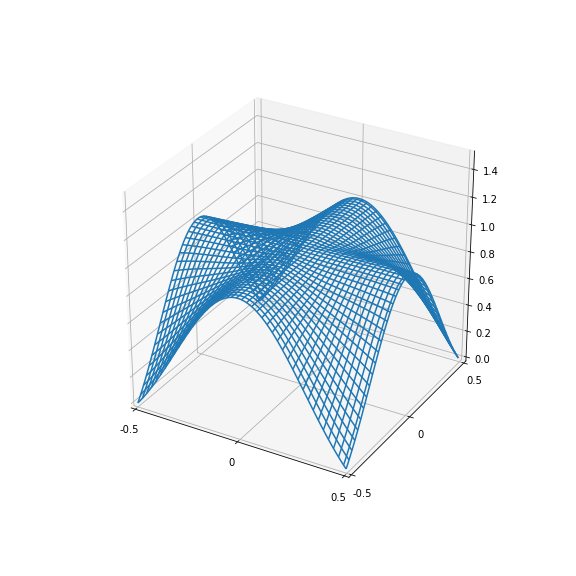
\includegraphics[width=0.8\linewidth]{pictures/variational/freq_char/3dpiece.png}}
\caption{Частотная характеристика при восстановлении по средним локальным апертурам значений наклонов.$ \alpha = 0.00001\,,\gamma = 0.1$.}
\label{ris:piece_plt}
\end{figure}
\begin{figure}[H]
\center{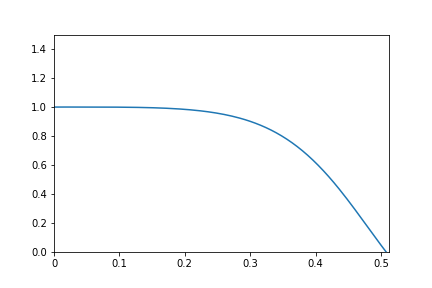
\includegraphics[width=0.5\linewidth]{pictures/variational/freq_char/2dpiece.png}}
\caption{Частотная характеристика $H_{ll}$ при восстановлении по средним локальным апертурам значений наклонов}
%\label{ris:cont_plt}
\end{figure}

Ниже приведена частотная характеристика $H_{ll}$ при $\alpha = 0.00001$ и различных $\gamma$.
\begin{figure}[H]
\center{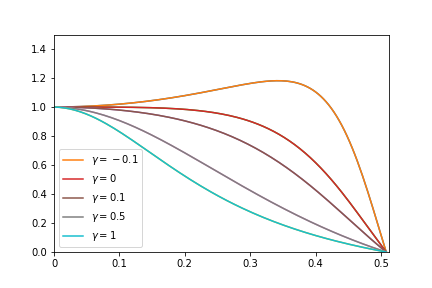
\includegraphics[width=0.6\linewidth]{pictures/variational/freq_char/2dpiece4vars.png}}
\caption{Частотная характеристика $H_{ll}$ при $\alpha = 0.00001$ и различных $\gamma$.}
\end{figure}
%\label{ris:cont_plt}


\subsection{Применение вариационного метода для восстановления полиномов Цернике}
Выполним восстановление полиномов $Z_3^{-1} = 3\rho^3 - 2\rho  \sin(\phi),\,Z_3^{3} = \rho^3  \cos(3\phi),\,Z_2^{-2} = \rho^2 \sin(2\phi)$ при различных $g_1, g_2$.
\subsubsection{Точные значения производных}
\begin{figure}[H]
\center{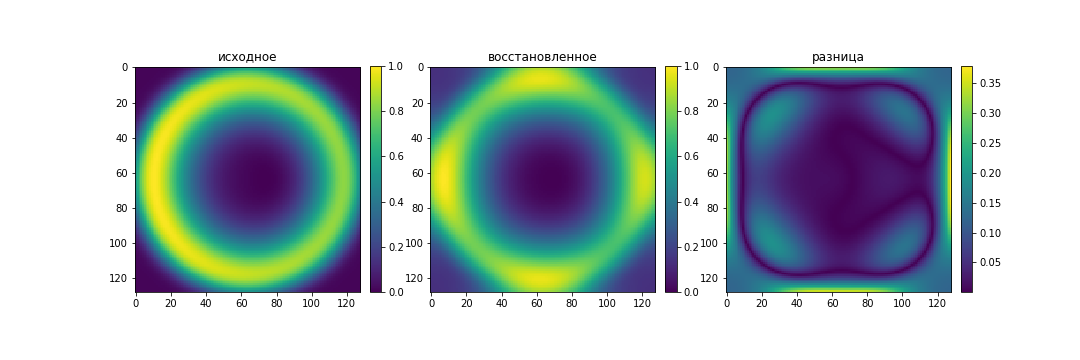
\includegraphics[width=1\linewidth]{pictures/variational/polys/z_3^-1.png}}
\caption{Полином $Z_3^{-1}$, $mse =3.504716747201833*10^{-6}$.}
\end{figure}
\begin{figure}[H]
\center{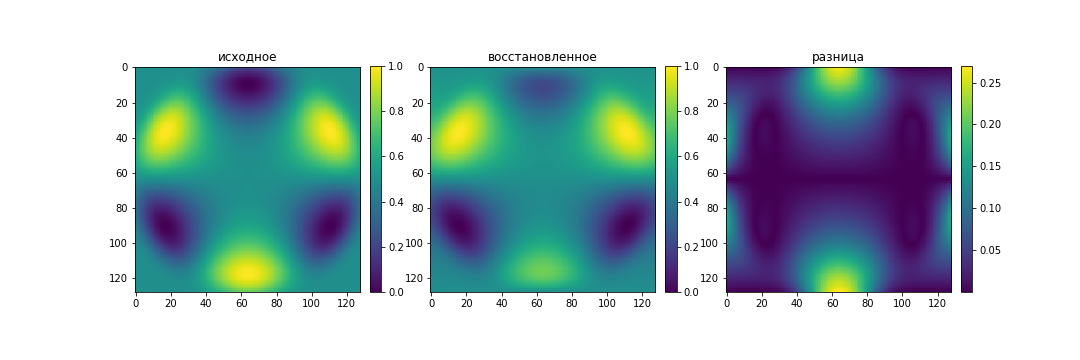
\includegraphics[width=1\linewidth]{pictures/variational/polys/z_3^3.png}}
\caption{Полином $Z_3^{3}$, $mse =1.6820583618382371*10^{-6}$.}
\end{figure}
\begin{figure}[H]
\center{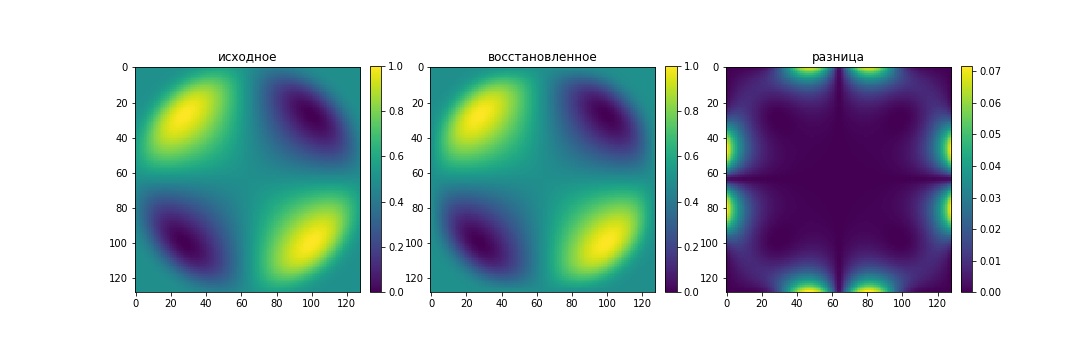
\includegraphics[width=1\linewidth]{pictures/variational/polys/z_2^-2.png}}
\caption{Полином $Z_2^{-2}$, $mse =1.1964663085490538*10^{-6}$.}
\end{figure}

\subsubsection{Случай восстановления по средним локальным апертурам значений наклонов}
\begin{figure}[H]
\center{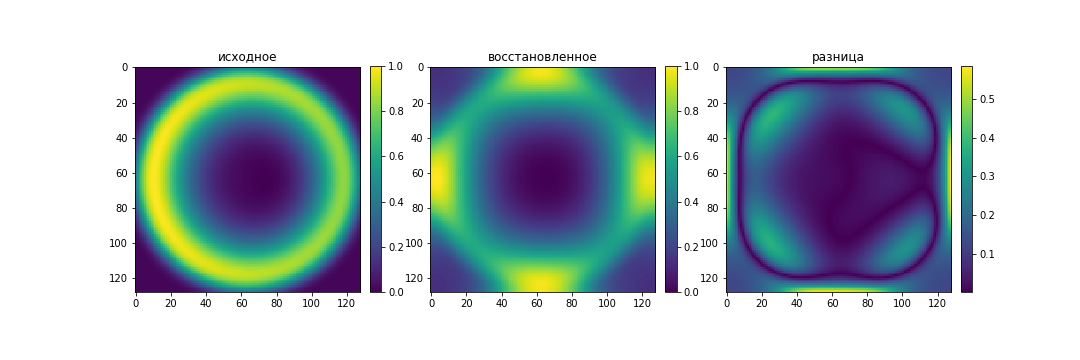
\includegraphics[width=1\linewidth]{pictures/variational/polys/z_3^-1_v2.png}}
\caption{Полином $Z_3^{-1}$, $mse = 0.00023758178351561665$.}
\end{figure}

\begin{figure}[H]
\center{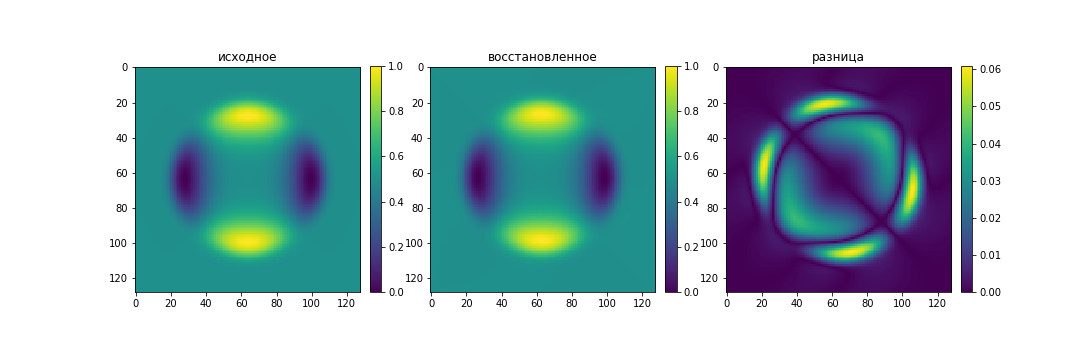
\includegraphics[width=1\linewidth]{pictures/variational/polys/z_3^3_v2.png}}
\caption{Полином $Z_3^{3}$, $mse =0.0001298752931746188$.}
\end{figure}

\begin{figure}[H]
\center{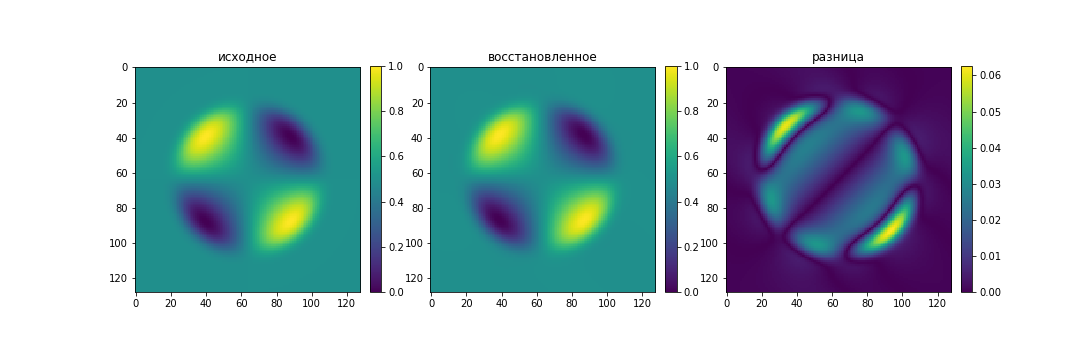
\includegraphics[width=1\linewidth]{pictures/variational/polys/z_2^-2_v2.png}}
\caption{Полином $Z_2^{-2}$, $mse =0.00010995511181308096$.}
\end{figure}
\newpage
\section*{Заключение}
В данной работе был исследован вейвлет метод восстановления волнового фронта, и проведено его сравнение с вариационным методом. Была продемонстрирована их работа при восстановлении поверхностей, заданных полиномами Цернике. Удалось установить, что эффективность вейвлет метода зависит от того, насколько близки наклоны к первым разностным производным вперед. Получена частотная характеристика вариационного метода для случая восстановления по средним локальным апертурам значений наклонов. Данная постановка является более приближенной к реальности,нежели использование точных значений производных  в узлах сетки. Показана возможность модификации вариационного метода для различных входных данных.

\addcontentsline{toc}{section}{Заключение}

\newpage
\bibliography{bibl}

\end{document}
